\documentclass[a4paper,10pt]{article}
\usepackage[top=3cm, bottom=3cm, left=3cm, right=3cm]{geometry}
\usepackage[spanish]{babel}
\spanishdecimal{.}
\selectlanguage{spanish}
\usepackage[spanish,onelanguage,ruled]{algorithm2e}
\usepackage[utf8]{inputenc}
\usepackage{graphicx}
\usepackage{caption}
\usepackage{subcaption}
\usepackage{hyperref}
\usepackage{verbatim}
\usepackage{amssymb}
\usepackage{mathtools}
\usepackage{amsmath}
\usepackage[natbibapa]{apacite}
\bibliographystyle{apacite}
%\usepackage[nottoc,numbib]{tocbibind}
\newcommand\ddfrac[2]{\frac{\displaystyle #1}{\displaystyle #2}}
\DeclareMathOperator{\atantwo}{atan2}

\title{Posiciones de los Planetas y la Luna \\ Macroproyecto para Matemáticas}
\author{Marco Negrete, Javier Alatorre, Daniela Madrigal y Melissa Santoyo}
\date{Proyecto Aleph 5}

\begin{document}
\renewcommand{\tablename}{Tabla}
\renewcommand{\BOthers}[1]{et al.\hbox{}}
\maketitle

\begin{abstract}
  Este documento contiene un resumen de los cálculos necesarios para estimar las posiciones de los primeros cinco planetas del sistema solar y la luna, vistos desde un punto dado sobre la Tierra, en una fecha y hora determinadas. También se incluyen instrucciones para escribir el código necesario, en los lenguajes Java y Python, para implementar estos cálculos en la aplicación StarGazer (para Android). Este documento va dirigido a los docentes y tiene como objetivo servir de apoyo, en la parte técnica, para facilitar la ejecución de la secuencia didáctica correspondiente. 
\end{abstract}

\section{Introducción}
Para este macroproyecto se considera que el movimiento de los planetas es Kepleriano, es decir, se considera que la órbita de los planetas es eclíptica y que su movimiento está determinado sólamente por la interacción gravitatoria entre el planeta en cuestión y el sol. Existen factores que alteran el movimiento de un planeta, como la gravedad de otros planetas y la presión de radiación solar, sin embargo, estos efectos son mínimos y para este macroproyecto no se tomaron en cuenta. 

Dados los supuestos anteriores, la posición de un planeta se puede estimar, a grandes rasgos, con los siguientes pasos:
\begin{enumerate}
\item Obtención de los parámetros orbitales (ya sea de los planetas o la Luna).
\item Cálculo de la posición del planeta con respecto al plano de su propia órbita.
\item Transformación de esta posición a coordenadas eclípticas y después a ecuatoriales.
\item Cálculo del tiempo sideral local.
\item Transformación de coordenadas ecuatoriales a coordenadas horizontales.
\end{enumerate}

Cada uno de los pasos anteriores corresponde a un día de trabajo en al secuencia didáctica. El paso final de la secuencia consiste en la programación de los cálculos para generar la aplicación móvil StarGazer. En las siguientes secciones se explican a detalle cada uno de estos cálculos.

\section{Antecedentes: parámetros orbitales}
Para definir qué son los parámetros orbitales, primero es necesario definir algunos sistemas de referencia. El primero de ellos es el sistema de coordenadas eclípticas. En este sistema, el plano $XY$ coincide con el plano de la órbita de la Tierra y el eje positivo de las $X$ (dirección primaria) apunta hacia el equinoccio vernal, es decir, hacia el punto en el que se encuentra el Sol, visto desde la Tierra, cuando ocurre el equinoccio de primavera en el hemisferio norte. En la figura \ref{fig:EclipticFrame} se muestra este sistema de coordenadas. En el sistema eclíptico, el origen puede fijarse en el Sol o en la Tierra, pero el plano $XY$ siempre coincide con el plano orbital de la Tierra y el eje $X$ apunta hacia el Primer Punto de Aries (como también se conoce la dirección en que se encuentra el Sol, visto desde la Tierra, en el equinoccio vernal). Lo más común, es utilizar el Sol como origen del sistema eclíptico. 
\begin{figure}
  \centering
  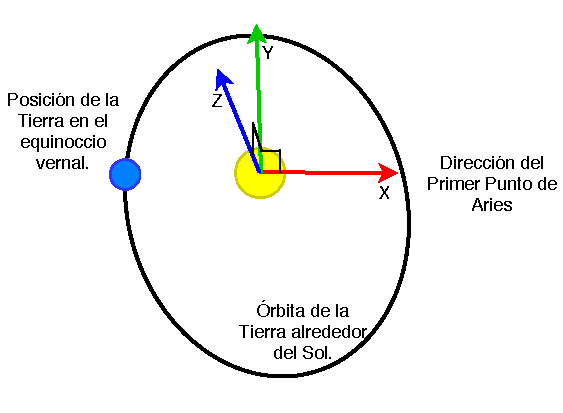
\includegraphics[width=0.5\textwidth]{Figures/EclipticCoordinates.pdf}
  \caption{Sistema de coordenadas eclípticas.}
  \label{fig:EclipticFrame}
\end{figure}

Las órbitas de todos los planetas son elipses con el Sol en uno de los focos, sin embargo, estas elipses no son coplanares con la órbita de la Tierra, no tienen la misma orientación en el espacio ni la misma ``forma'' y tamaño. Por ello se requieren tres parámetros (ángulos) para definir la orientación de la órbita en el espacio y dos más para definir su forma y tamaño. Una vez definida la forma y orientación de la órbita, un sexto parámetro se utiliza para definir la posición del planeta en un momento determinado. Estos seis parámetros son conocidos como los parámetros orbitales. A continuación se describen más a detalle cada uno de ellos.

\subsection{Excentricidad y semieje mayor}
Como se mencionó anteriormente, estos dos parámetros sirven para definir la forma y tamaño de la órbita de un planeta. Es importante recordar dos conceptos: el perihelio y el afelio. El perihelio de un planeta ocurre cuando este se encuentra más cerca del Sol, a una distancia $d_p$, y el afelio, cuando se encuentra más lejos, a una distancia $d_a$. Estos dos puntos también se conocen como periápside y apoápside. La longitud del semieje mayor $a$ es la distancia del centro de la elipse a cualquiera de los ápsides y es también igual a la distancia media del planeta al sol, es decir:
\[a = \frac{d_a + d_p}{2}\]
La distancia $c$ corresponde a la distancia desde el centro de la elipse a cada uno de los focos, es decir, del centro de la órbita al Sol. En la figura \ref{fig:Ellipse} se muestran cada una de estas distancias. La excentricidad de la órbita se puede calcular como:
\begin{equation}
  e = \frac{c}{a}
  \label{eq:Eccentricity}
\end{equation}
Para las elipses, este cociente siempre es mayor que cero y menor que uno. Entre más pequeña sea la excentricidad, la órbita se parece más a un círculo. Otra relación importante es la que existe entre el semieje mayor $a$, el semieje menor $b$ y la excentricidad $e$, dada por:
\begin{equation}
  b = a\sqrt{1 - e^2}
  \label{eq:Semiaxis}
\end{equation}

Para caracterizar la forma y tamaño de la elipse, se podrían usar la excentricidad y cualquiera de las distancias indicadas en la figura \ref{fig:Ellipse}. Lo más común es usar $e$ y $a$ para este fin. La excentricidad $e$ es adimensional mientras que la distancia $a$ se suele medir en unidades astronómicas (AU por sus siglas en inglés) para los planetas, y en radios de la Tierra (ER por sus siglas en inglés) para la Luna. Una unidad astronómica se define como la distancia media de la Tierra al Sol, es decir, para la órbita de la Tierra, por definición, $a=1$.
\begin{figure}
  \centering
  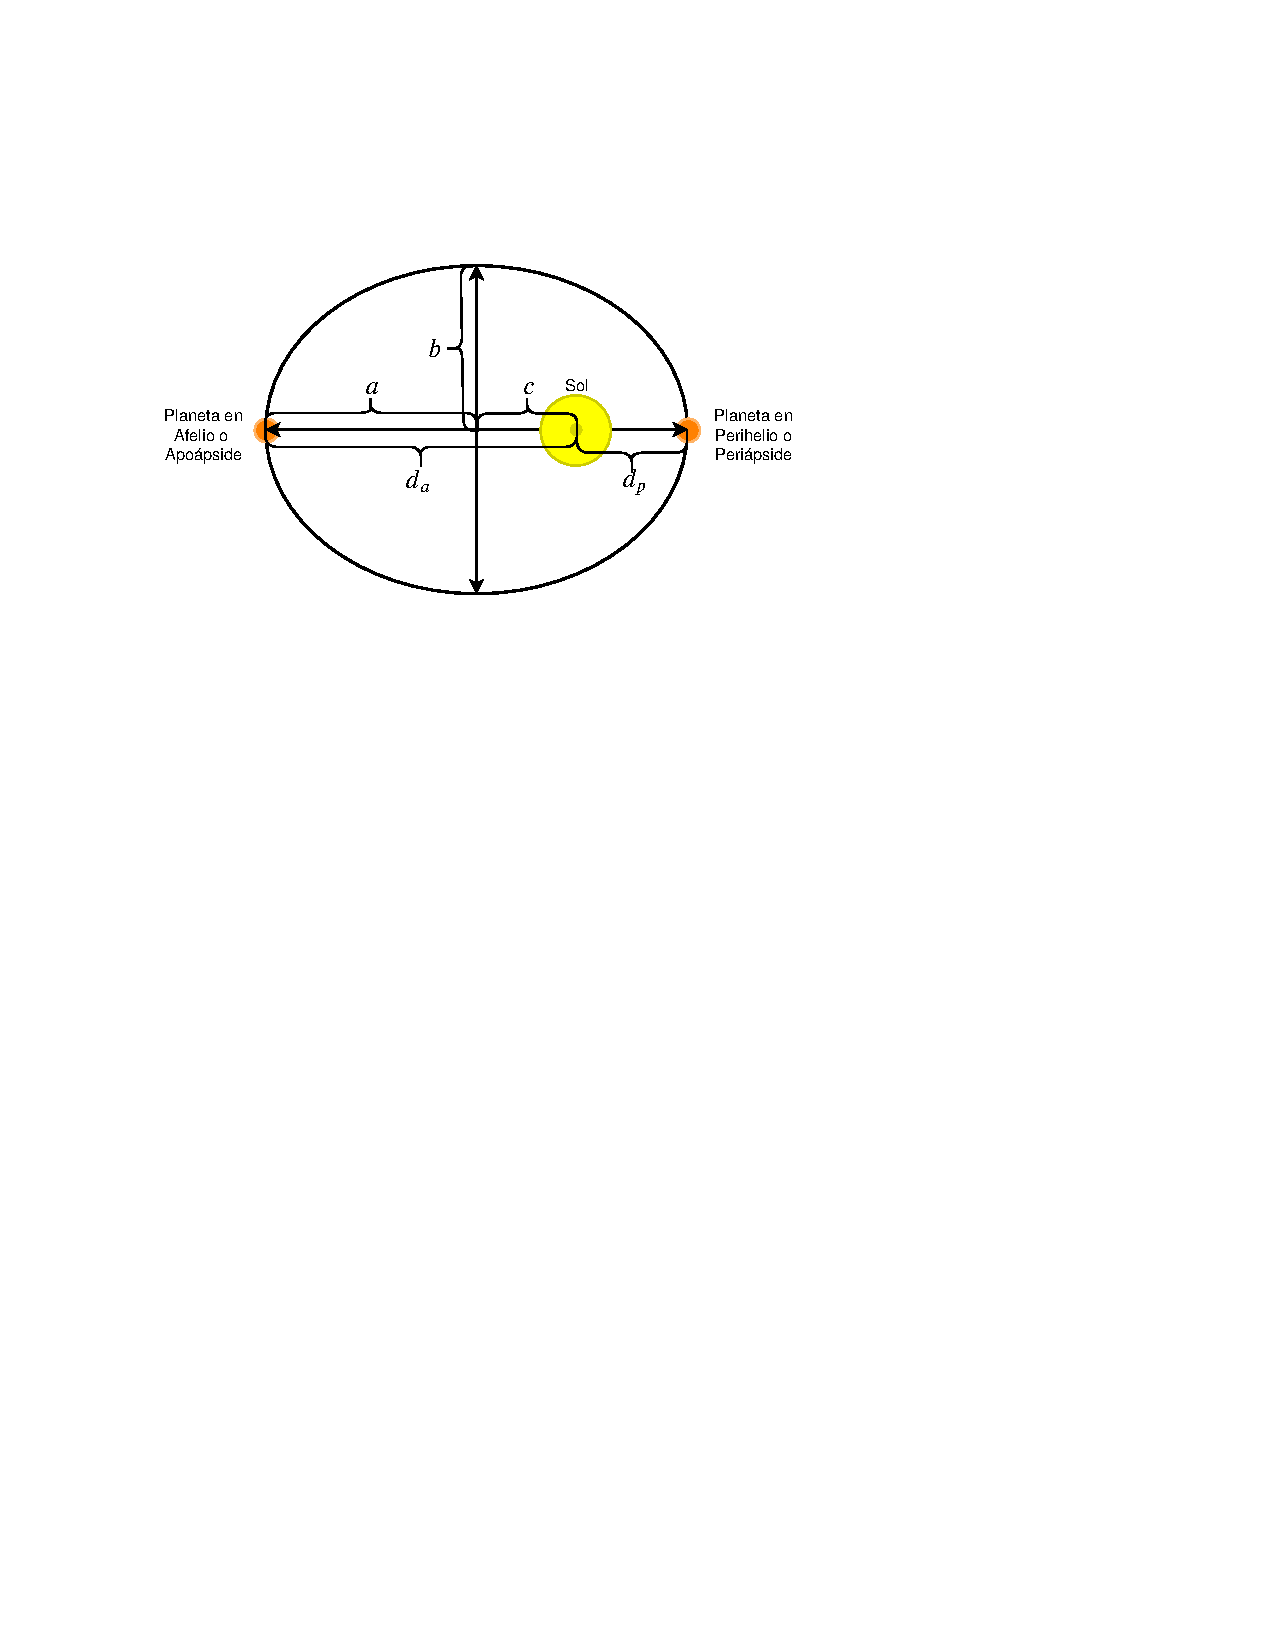
\includegraphics[width=0.6\textwidth]{Figures/EccentricitySemimajorAxis.pdf}
  \caption{Medidas importantes en la órbita de un planeta. Las distancias $a$, $b$, $c$, $d_p$ y $d_a$ se miden en unidades astronómicas.}
  \label{fig:Ellipse}
\end{figure}

\subsection{Orientación de la órbita: ángulos $N$, $i$ y $\omega$}
\label{sec:NiwAngles}
Para definir la orientación de un objeto en el espacio se requieren siempre de cuando menos tres parámetros. Para las órbitas planetarias, estos tres parámetros corresponden a tres ángulos: longitud del nodo ascendente $N$, inclinación $i$ y argumento del periápside $\omega$, los cuales sirven para expresar la orientación de la órbita de un planeta con respecto al sistema de coordenadas eclípticas. Para explicar estos ángulos, considere los dos sistemas coordenados mostrados en la figura \ref{fig:Niw}. Uno de ellos es el sistema eclíptico $O_E$ (con dirección primaria hacia el Primer Punto de Aries y coplanar con la órbita de la Tierra) y el otro es el sistema $O_P$, cuyo plano $X_P Y_P$ es paralelo a la órbita del planeta en cuestión y cuya dirección primaria (dirección del eje positivo de $X_P$) apunta hacia el perihelio de dicho planeta. En la figura \ref{fig:Niw} se muestran los dos sistemas de referencia y los tres ángulos $N$, $i$ y $\omega$.

\begin{figure}
  \centering
  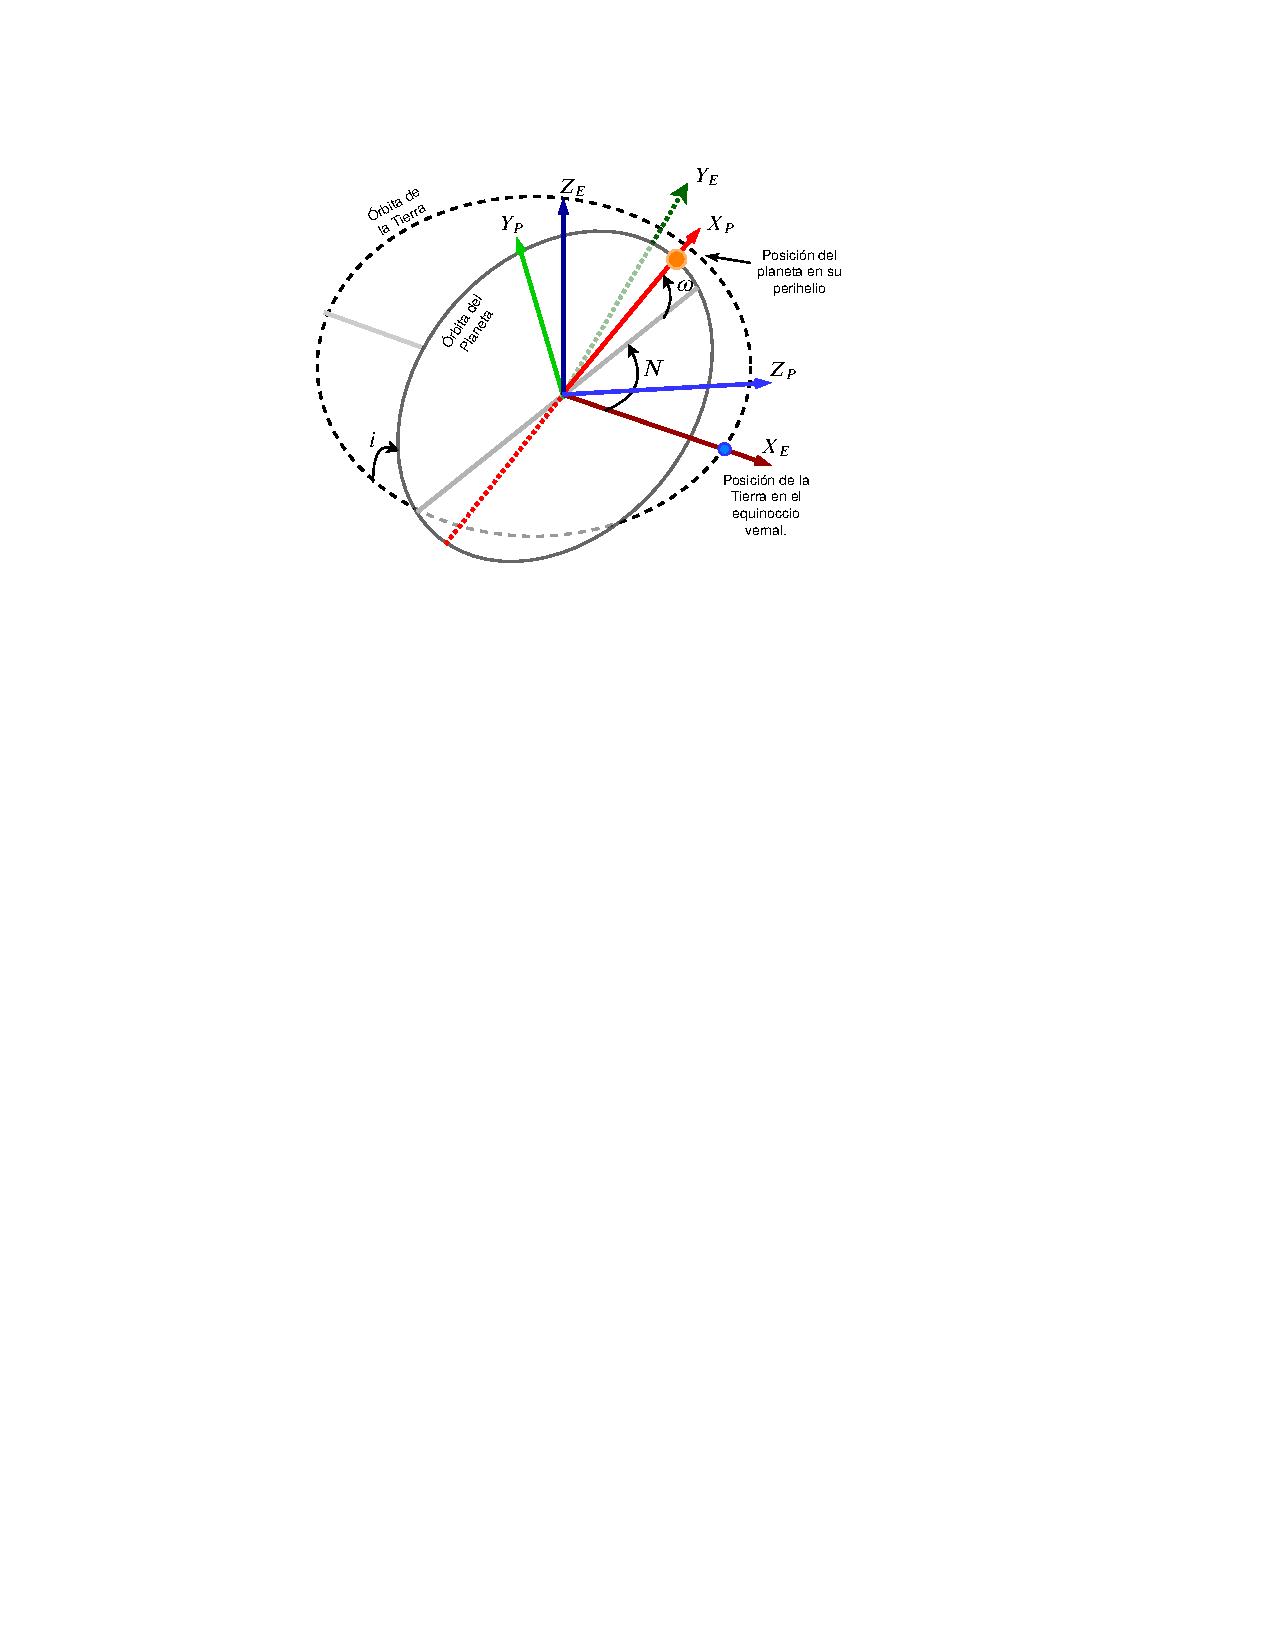
\includegraphics[width=0.6\textwidth]{Figures/Niw.pdf}
  \caption{Ángulos y sistemas de referencia para definir la orientación de la órbita de un planeta.}
  \label{fig:Niw}
\end{figure}

Tanto el sistema de referencia $O_P$ (el de la órbita del planeta) como el $O_E$ (el de la órbita de la Tierra) tienen como centro el Sol, pero el sistema $O_P$ está rotado con respecto a $O_E$, es decir, $O_P$ se puede obtener rotando $O_E$ primero un ángulo $N$ sobre el eje $Z$, luego un ángulo $i$ sobre el eje $X$ y finalmente un ángulo $\omega$ nuevamente sobre el eje $Z$. En otras palabras, la orientación de la órbita de un planeta se puede obtener aplicando estas mismas rotaciones a la órbita de la Tierra. En la figura \ref{fig:Rotations} se muestran paso por paso estas rotaciones.
\begin{figure}
  \centering
  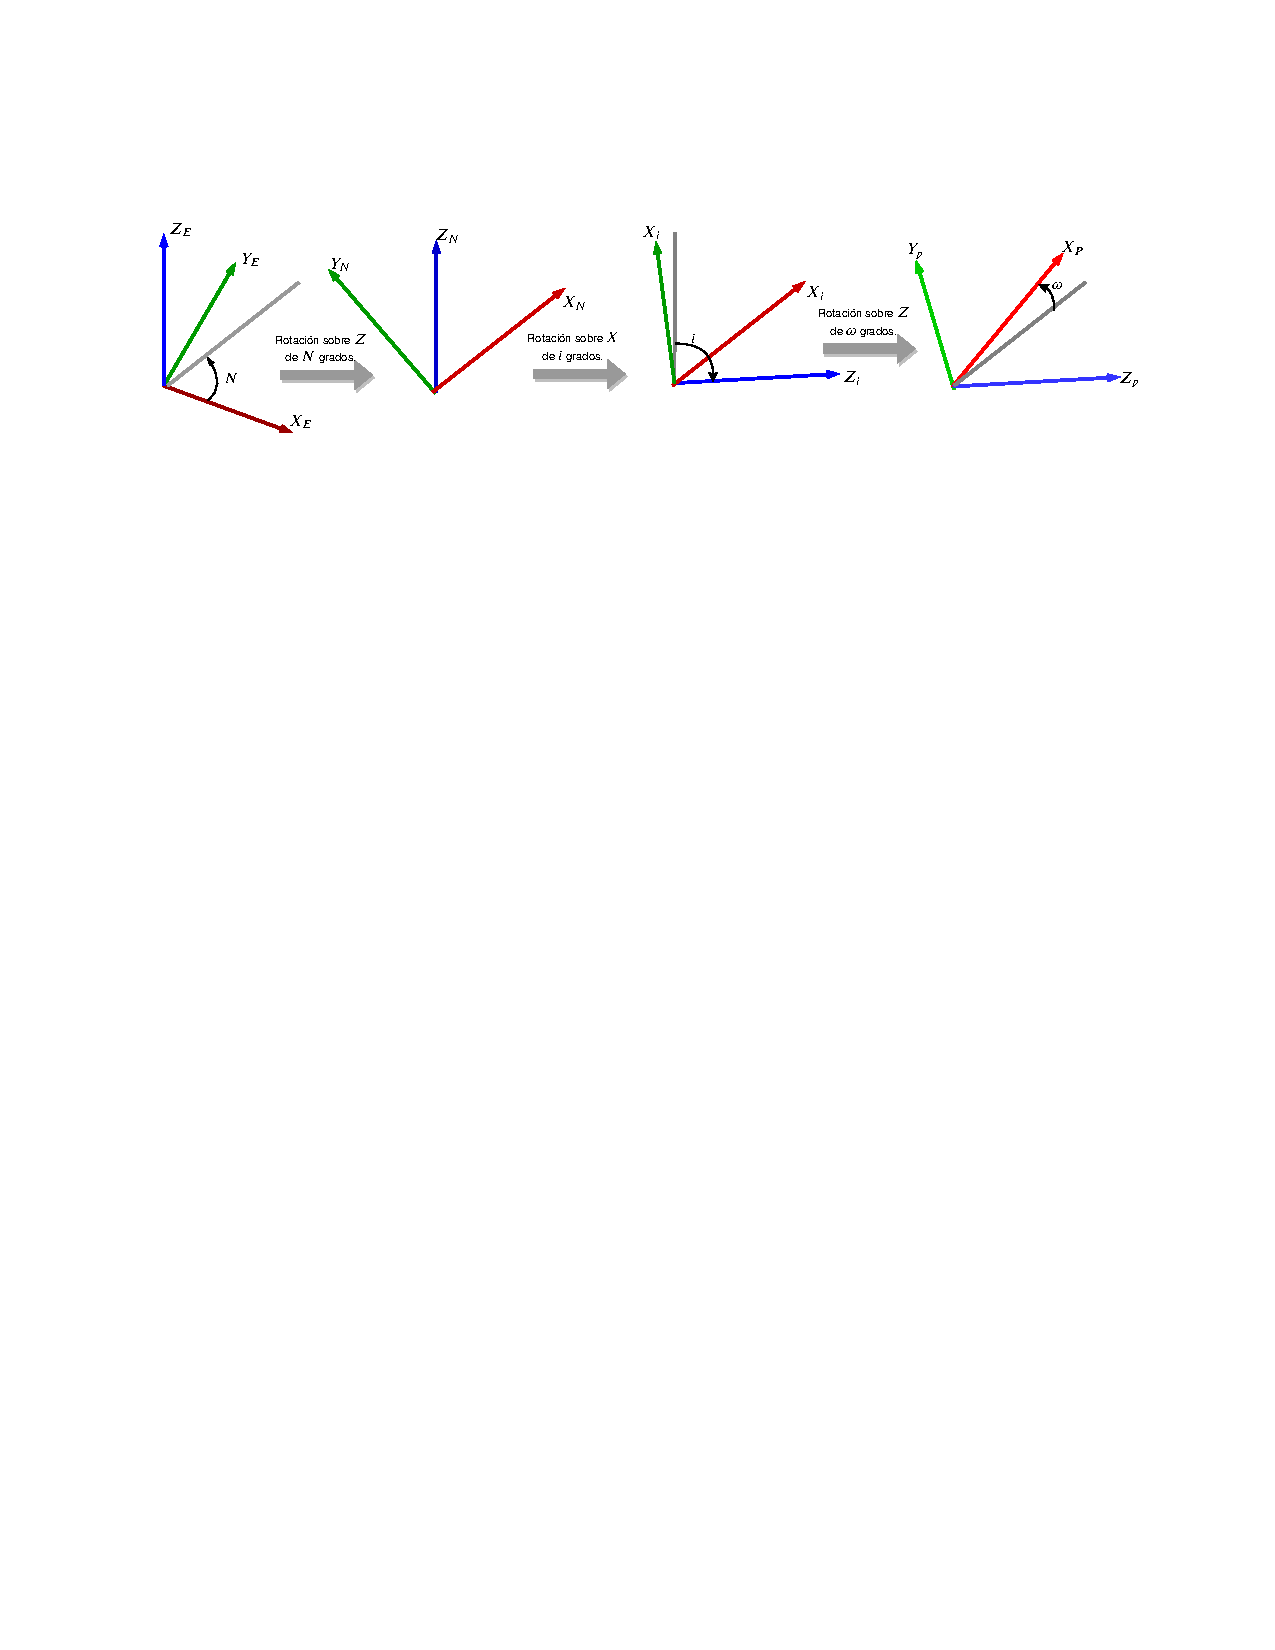
\includegraphics[width=\textwidth]{Figures/Rotations.pdf}
  \caption{Rotaciones para obtener $O_P$ a partir de $O_E$.}
  \label{fig:Rotations}
\end{figure}

\subsection{Anomalía media $M$}
De acuerdo con la Segunda Ley de Kepler, la velocidad angular de un planeta no es constante, siendo esta mayor en el perihelio y menor en el afelio. Sin embargo, a cada planeta se le puede asociar una órbita circular imaginaria con el mismo periodo y con un radio igual al semieje mayor de la órbita real. En esta órbita imaginaria circular, el planeta tendría una velocidad angular constante y, por lo tanto, su posición en dicha órbita se podría caracterizar con un sólo parámetro. A este parámetro se le conoce como anomalía media $M$ y corresponde al ángulo del planeta medido desde su perihelio hacia la posición sobre la órbita circular imaginaria. En la figura \ref{fig:MeanAnomaly} se muestra la forma de medir este ángulo.

\begin{figure}
  \centering
  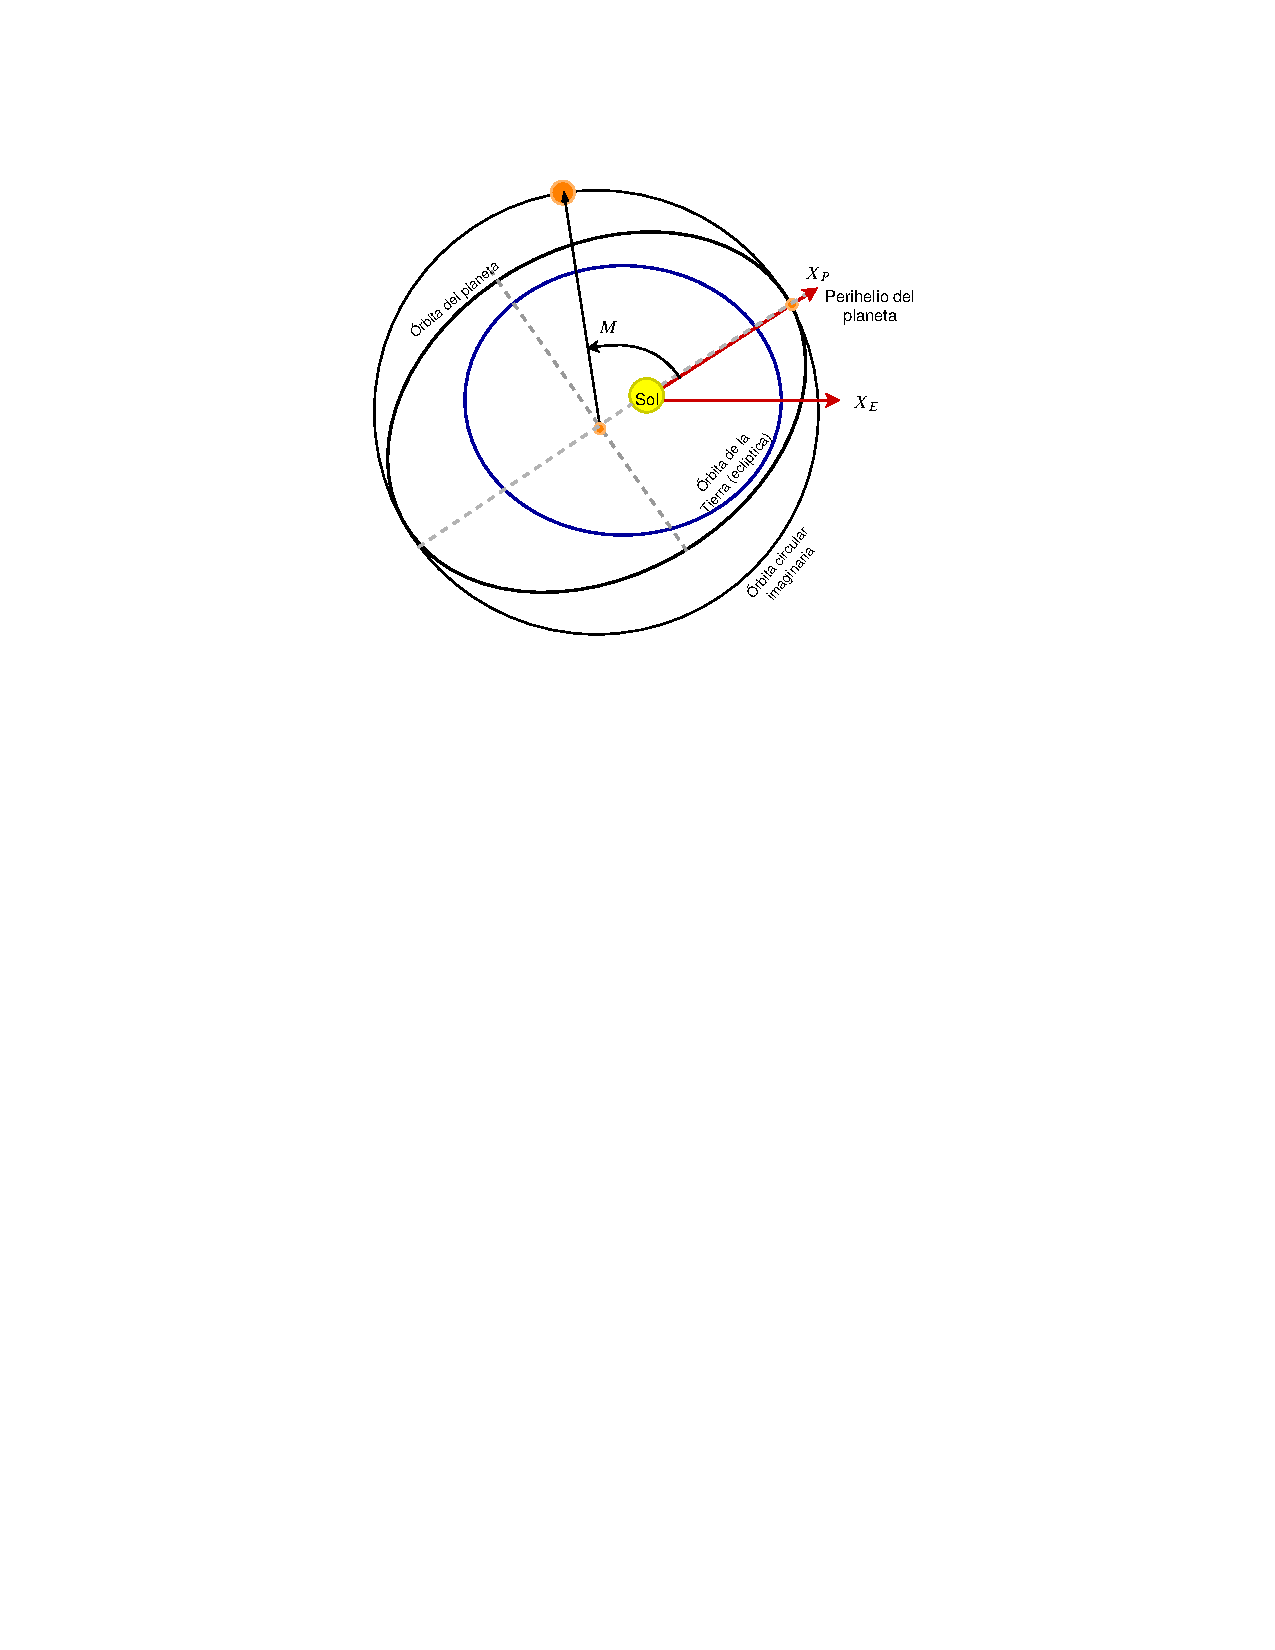
\includegraphics[width=0.5\textwidth]{Figures/MeanAnomaly.pdf}
  \caption{Anomalía media $M$.}
  \label{fig:MeanAnomaly}
\end{figure}

Resumiendo, los seis parámetros orbitales son:
\begin{itemize}
  \item Para la forma y tamaño de la órbita:
  \begin{itemize}
  \item \textbf{$a$}: semieje mayor, medido en en AU para los planetas y en ER para la Luna.
  \item \textbf{$e$}: excentricidad, adimensional.
  \end{itemize}
  \item Para la orientación de la órbita con respecto a la eclíptica:
  \begin{itemize}
  \item \textbf{$N$}: longitud del nodo ascendente (rotación sobre $Z$).
  \item \textbf{$i$}: inclinación de la órbita (rotación sobre $X$).
  \item \textbf{$\omega$}: argumento del periápside (rotación sobre $Z$). 
  \end{itemize}
  \item Para la posición del planeta sobre su propia órbita:
  \begin{itemize}
  \item \textbf{$M$}: anomalía media, que se mide a partir del perihelio del planeta (ver figura \ref{fig:MeanAnomaly}).
  \end{itemize}
\end{itemize}


\section{Día 1: Determinar los parámetros orbitales}
A excepción de la anomalia media, los parámetros orbitales se pueden considerar constantes para periodos cortos de tiempo (años e incluso décadas), sin embargo, para mejorar las estimaciones de posición, se tomarán en cuenta las pequeñas variaciones a lo largo del tiempo. Una buena aproximación para los parámetros orbitales es calcularlos en función del tiempo mediante una ecuación de primer grado, es decir, si se grafica cada parámetro con respecto al tiempo, se obtendría una recta. Para este trabajo los parámetros orbitales se calculan como se indica en la tabla \ref{tab:OrbitalParams}. Es importante recordar que el semieje mayor se mide en unidades astronómicas para los planetas y en radios de la Tierra para la Luna. Además, para todos los planetas se considera que el sistema eclíptico tiene origen en el Sol, mientras que para la Luna, se considera el origen en la Tierra. 
\begin{table}
  \centering
  \begin{tabular}{cll}
    \hline
    Parámetro & Luna & Mercurio \\
    \hline
    $a     $ & $60.2666                  $  & $0.387098                $ \\
    $e     $ & $0.054900                 $  & $0.205635 + 5.59E-10d    $ \\
    $N     $ & $125.1228 - 0.0529538083d $  & $48.3313 + 3.24587E-5d   $ \\
    $i     $ & $5.1454                   $  & $7.0047 + 5.00E-8d       $ \\
    $\omega$ & $318.0634 + 0.1643573223d $  & $29.1241 + 1.01444E-5d   $ \\
    $M     $ & $115.3654 + 13.0649929509d$  & $168.6562 + 4.0923344368d$ \\
    \hline      
              & Venus & Tierra \\
    $a     $ & $0.723330               $  & $1.000000                $ \\
    $e     $ & $0.006773 - 1.302E-9d   $  & $0.016709 - 1.151E-9d    $ \\
    $N     $ & $76.6799 + 2.46590E-5d  $  & $0.0                     $ \\
    $i     $ & $3.3946 + 2.75E-8d      $  & $0.0                     $ \\
    $\omega$ & $54.8910 + 1.38374E-5d  $  & $102.9404 + 4.70935E-5d  $ \\
    $M     $ & $48.0052 + 1.6021302244d$  & $356.0470 + 0.9856002585d$ \\
    \hline
              & Marte & Júpiter \\
    $a     $ & $1.523688               $  & $5.20256                $ \\
    $e     $ & $0.093405 + 2.516E-9d   $  & $0.048498 + 4.469E-9d   $ \\
    $N     $ & $49.5574 + 2.11081E-5d  $  & $100.4542 + 2.76854E-5d $ \\
    $i     $ & $1.8497 - 1.78E-8d      $  & $1.3030 - 1.557E-7d     $ \\
    $\omega$ & $286.5016 + 2.92961E-5d $  & $273.8777 + 1.64505E-5d $ \\
    $M     $ & $18.6021 + 0.5240207766d$  & $19.8950 + 0.0830853001d$ \\
    \hline
              & Saturno & \\
    $a     $ & $9.55475                 $  & $ $ \\
    $e     $ & $0.055546 - 9.499E-9d    $  & $ $ \\
    $N     $ & $113.6634 + 2.38980E-5d  $  & $ $ \\
    $i     $ & $2.4886 - 1.081E-7d      $  & $ $ \\
    $\omega$ & $339.3939 + 2.97661E-5d  $  & $ $ \\
    $M     $ & $316.9670 + 0.0334442282d$  & $ $ \\
    \hline
  \end{tabular}
  \caption{Ecuaciones para el cálculo de los parámetros orbitales. Los ángulos están dados en grados.}
  \label{tab:OrbitalParams}
\end{table}

En las ecuaciones de la tabla \ref{tab:OrbitalParams} el tiempo $d$ se mide en días contados a partir de las 00:00:00 hrs del 31 de diciembre de 1999 en el horario del Timepo Universal Coordinado (UTC) (que coincide con la hora del Meridiano Greenwich). Por ejemplo, si se desean calcular los parámetros orbitales para el 10 de enero de 2000 a las 6:00 am en la hora de la Ciudad de México, se tendría que realizar lo siguiente: primero, las 6:00 am de la Ciudad de México, en horario de invierno, corresponde con las 12:00 hrs en UTC. Desde las 00:00 hrs del 31 de diciembre de 1999 hasta las 12:00 hrs del 10 de enero de 2000, han pasado 10 días con 12 horas, por lo tanto, los parámetros orbitales, para el 10-01-2000 a las 6:00 am hora de la Cd Mx, se deben calcular considerando $d=10.5$.

En un ejemplo más complejo, si se desean calcular los parámetros para el 13 de sep de 2019 (día del programador) a las 8:00 am se debe realizar los siguiente: entre 1999 y 2019 hubo 5 años bisiestos, por lo que el número de días transcurridos hasta las 00:00 hrs del 31 de diciembre de 2018 fueron 6940. El 13 de sep de 2019 fue el día número 256 del año, por lo que, desde las 00:00 hrs del 31-12-1999 hasta las 00:00 hrs del 13-19-2019, transcurrieron 7196 días exactos. Las 8:00 am en la CdMx en horario de verano corresponden con las 13:00 hrs  en UTC. 13 horas son 0.5416 días, por lo que los parámetros orbitales se deberían calcular con $d=7196.5416$. Las ecuaciones de la tabla \ref{tab:OrbitalParams} son válidas para fechas anteriores al 01-12-1999, para las cuales el tiempo $d$ sería negativo. 

\subsection{Timestamps}
En el ejemplo anterior, resulta muy laborioso calcular el número de días transcurridos, debido a la irregularidad de la duración de los meses y años, sin embargo, para este macroproyecto, se tiene la ventaja de implementarse en un dispositivo de cómputo móvil. Las computadoras llevan un registro de tiempo utilizando lo que se conoce como \textit{timestamp}. Un \textit{timestamp} es un número entero que indica el número de segundos transcurridos desde las 00:00:00 hrs GMT del 1 de enero de 1970. A diferencia de los años y meses, los días sí tienen una duración constante, que es de 86400 segundos; por lo tanto, si se divide un timestamp entre 86400 se tendrá el número de días transcurridos desde el 1 de enero de 1970. Si a un timestamp se le resta el timestamp correspondiente al 31-12-1999 a las 00:00 hrs, y esta diferencia se divide entre 86400, se obtendrán los días transcurridos como se requiere en las ecuaciones de la tabla \ref{tab:OrbitalParams}:
\begin{equation}
  d = \frac{t_c - t_s}{86400}
  \label{eq:ElapsedDays}
\end{equation}
donde
\begin{eqnarray*}
  t_c &:& \textrm{Timestamp de la fecha y hora de interés}\\
  t_s &:& \textrm{Timestamp del 31 de diciembre de 1999 a las 00:00:00 hrs GMT}
\end{eqnarray*}
Obtener el número de segundos transcurridos a partir de una fecha parece algo aún más laborioso que obtener los días transcurridos, sin embargo, todos los dispositivos de cómputo llevan este conteo y es muy sencillo obtenerlo; por ejemplo, para dispositivos con Android, existe la función \texttt{System.currentTimeMillis()} que obtiene el \textit{timestamp} actual. Existen también herramientas en línea para la obtención de timestamps, por ejemplo \url{https://www.epochconverter.com/}

En síntesis, los cálculos del día 1 de la secuencia didáctica se pueden resumir en la obtención de los parámetros orbitales de acuerdo con la tabla \ref{tab:OrbitalParams} y el cálculo de días transcurridos de acuerdo con la ecuación \ref{eq:ElapsedDays}.

\section{Día 2: Posición del planeta sobre su propia órbita}
Para calcular la posición del planeta con respecto a su propia órbita se considerará un sistema de referencia $O_P$ cuyo eje $X$ apunta hacia su perihelio, el eje $Z$ apunta hacia lo que sería el ``norte'' geográfico del planeta, y el eje $Y$, orientado de modo que el sistema sea dextrógiro. Las figuras \ref{fig:Niw} y \ref{fig:MeanAnomaly} muestran la orientación del sistema de referenica $O_P$.

Una vez definido el sistema de referencia $O_P$, es necesario definir otros dos conceptos: anomalía verdadera y anomalía excéntrica. Para definirlos, es necesario retomar el concepto de anomalía media, que es la posición del planeta sobre una órbita circular imaginaria de radio igual al semieje mayor y periodo igual a la órbita real.

Considere el esquema mostrado en la figura \ref{fig:Anomalies}. $P_M$ es la posición del planeta sobre una órbita circular imaginaria y que se determina mediante la anomalía media, que es uno de los seis parámetros orbitales. La posición $P'$ es también una posición sobre una órbita circular imaginaria. El ángulo entre el eje $X$ y el vector de posición $P'$ se conoce como anomalía excéntrica $E$. La relación entre la anomalía media $M$ y la anomalía excéntrica $E$ está dada por la Ecuación de Kepler:
\begin{equation}
  M = E - e\sin E
  \label{eq:Kepler}
\end{equation}
donde $e$ es la excentricidad de la órbita. En la siguiente subsección se aborda la solución de esta ecuación. Finalmente, la anomalía verdadera $V$ es el ángulo entre el eje $X$ y la posición real del planeta, tomando como origen el Sol y no el centro de la órbita (el Sol está en uno de los focos). La relación entre las anomalías excéntrica y verdadera está dada por las propiedades geométricas de la elipse. 
\begin{figure}
  \centering
  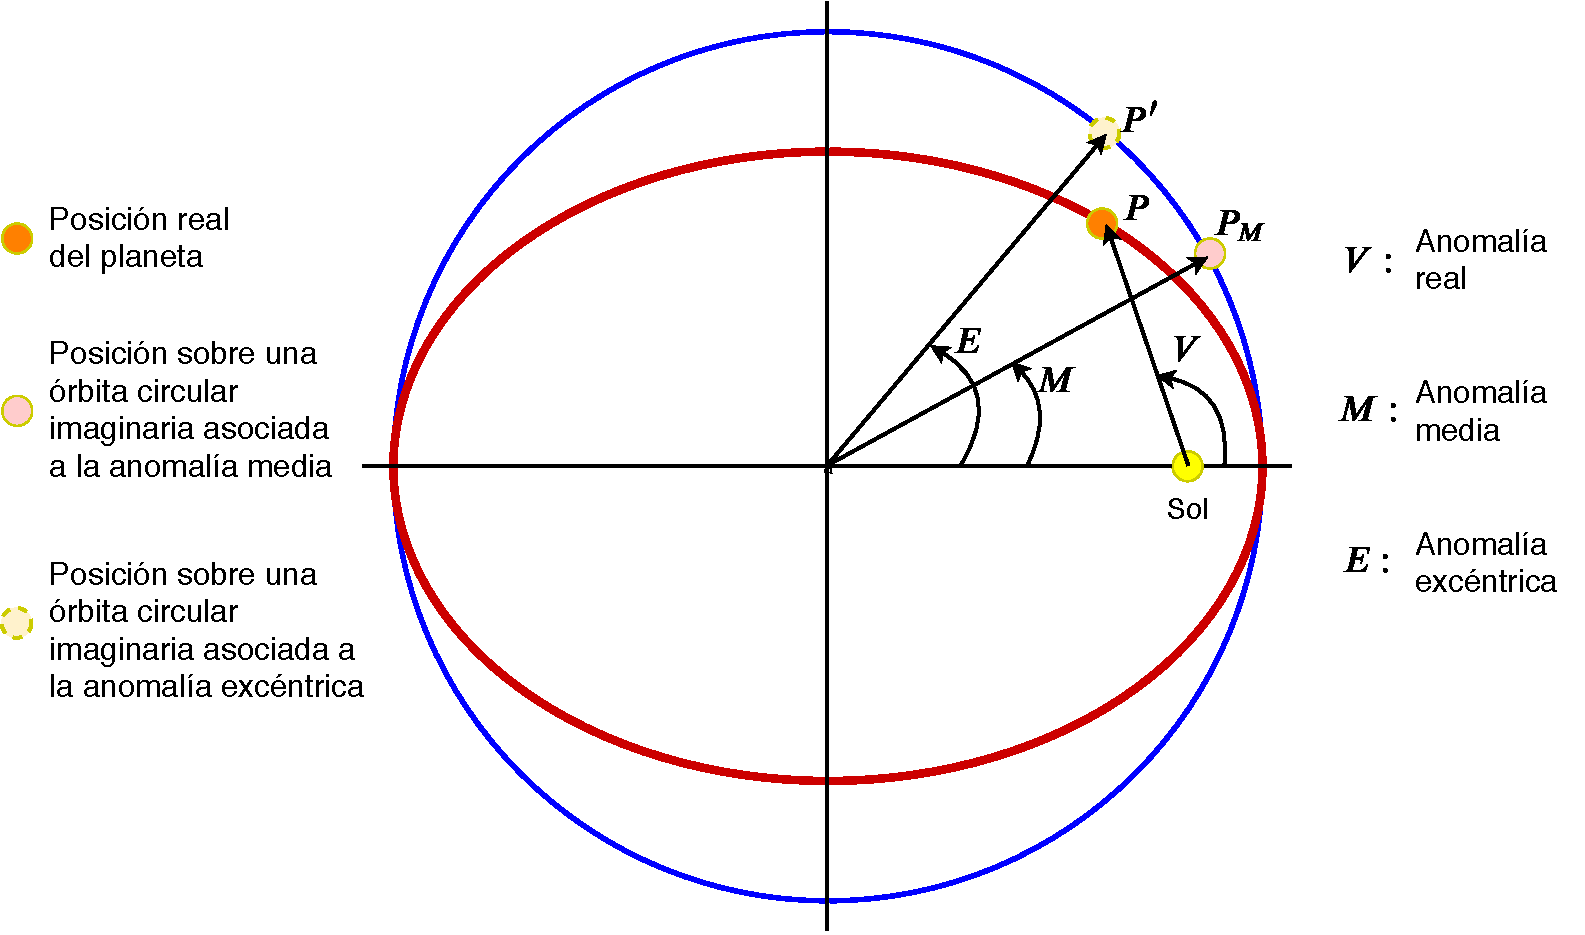
\includegraphics[width=0.75\textwidth]{Figures/Anomalies.pdf}
  \caption{Anomalías media, excéntrica y verdadera.}
  \label{fig:Anomalies}
\end{figure}

\subsection{Solución de la Ecuación de Kepler}

De acuerdo con la ecuación (\ref{eq:Kepler}), la obtención de la anomalía media a partir de la excéntrica es trivial, sin embargo, lo que se desea es lo contrario, obtener la anomalía excéntrica a partir de la media (que se obtiene de acuerdo con la tabla \ref{tab:OrbitalParams} y la ecuación (\ref{eq:ElapsedDays})). Para esto, sería necesario resolver (\ref{eq:Kepler}) para $E$, sin embargo, no existe una forma cerrada para la solución, es decir, es necesario obtener $E$ por un método numérico.

El método de Newton-Raphson sirve para encontrar raíces, es decir, para resolver ecuaciones de la forma:
\begin{equation}
  f(x) = 0
  \label{eq:NewtonRaphsonForm}
\end{equation}
El método se puede entender mejor si se considera la interpretación geométrica de la derivada. Considere la figura \ref{fig:NewtonRaphson}. Se tiene una curva dada por la función $f(x)$ y se desea encontrar el valor de $x$ en el que la curva cruza por cero, es decir, el valor $x_r$ que hace que se cumpla la ecuación $f(x) = 0$. Suponga que se tiene una estimación inicial $x_0$. Si se evalúa la derivada $f'(x)$ en $x_0$ se tiene la pendiente $m$ de la recta tangente a la curva $f(x)$ en $x_0$, es decir $m=f'(x_0)$. En la figura se puede observar que la pendiente $m$ también se puede calcular como
\[m = \frac{f(x_0)}{x_0 - x_1}\]
por lo tanto
\[f'(x_0) = \frac{f(x_0)}{x_0 - x_1}\]
de donde se obtiene que:
\begin{equation}
  x_1 = x_0 - \frac{f(x_0)}{f'(x_0)}
  \label{eq:NewtonRaphson}
\end{equation}
donde $x_1$ es una mejor aproximación a la solución de la ecuación (\ref{eq:NewtonRaphsonForm}). Si ahora $x_1$ se toma como una nueva $x_0$ y se vuelve a calcular $x_1$ de acuerdo con (\ref{eq:NewtonRaphson}) se obtendrá una mejor aproximación a la solución de (\ref{eq:NewtonRaphsonForm}). Si este proceso se repite un número suficiente de veces, el valor de $x_1$ puede considerarse como solución a la ecuación (\ref{eq:NewtonRaphsonForm}). A este proceso se le conoce como el método de Newton-Raphson. 
\begin{figure}
  \centering
  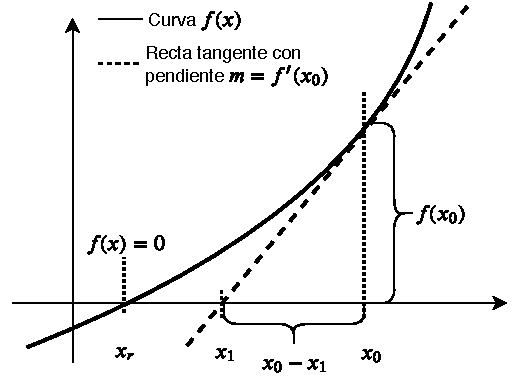
\includegraphics[width=0.6\textwidth]{Figures/GeometricDerivate.pdf}
  \caption{Método de Newton-Raphson.}
  \label{fig:NewtonRaphson}
\end{figure}

Para resolver la ecuación de Kepler por Newton-Raphson, primero se debe expresar (\ref{eq:Kepler}) en la forma (\ref{eq:NewtonRaphsonForm}):
\[
  f(E) = E - e\sin E - M = 0
\]
Derivando $f(E)$ con respecto a $E$ se obtiene:
\[
  f'(E) = 1 - e\cos E
\]
por lo que, dada una aproximación inicial $E_0$ para la solución de la Ecuación de Kepler, la siguiente aproximación $E_1$ se obtiene como:
\begin{equation}
  E_1 = E_0 - \frac{E_0 - e\sin E_0 - M}{1 - e\cos E_0}
  \label{eq:KeplerNumeric}
\end{equation}
Se mencionó que si el proceso se repite un número suficiente de veces, se llegará a la solución correcta. Para determinar que (\ref{eq:KeplerNumeric}) ya se ha ejecutado un número suficiente de veces, se puede calcular la diferencia del valor de $E_1$ entre una iteración y otra. Cuando esta diferencia sea menor que una tolerancia, se puede considerar que ya se ha encontrado el valor de $E$. Puesto que $E$ es un ángulo, es decir su valor está en el intervalo  $[0, 2\pi]$, una tolerancia adecuada puede ser algún valor en el orden de $10^{-6}$ o menor.

\begin{figure}
  \centering
  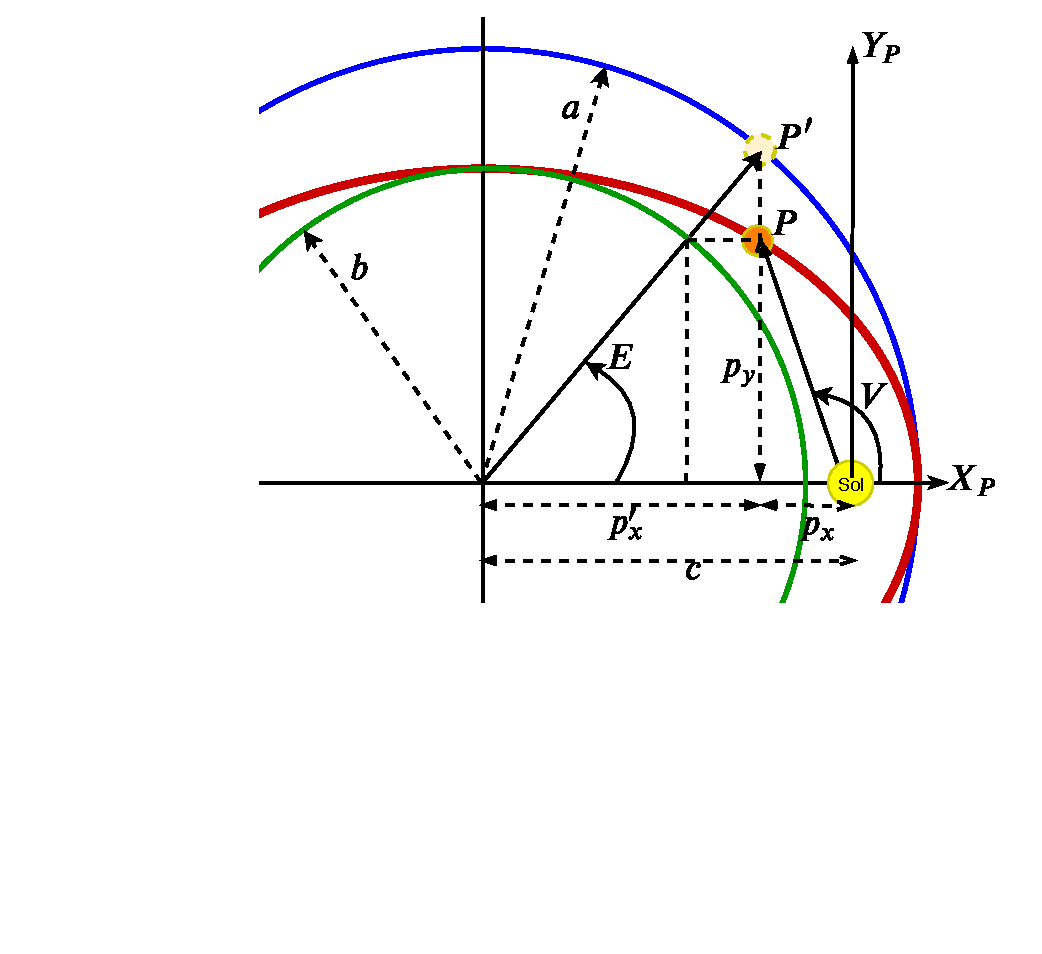
\includegraphics[width=0.6\textwidth]{Figures/AnomaliesEV.pdf}
  \caption{Relación entre las anomalías excéntrica $E$ y verdadera $V$.}
  \label{fig:AnomaliesEV}
\end{figure}
Una vez calculada la anomalía excéntrica $E$, se puede calcular la anomalía verdadera $V$ y la posición del planeta con respecto a su órbita. Considere el esquema de la figura \ref{fig:AnomaliesEV}, que muestra la relación entre las anomalías excéntrica y verdadera. De acuerdo con el esquema, la posición del planeta $(p_x, p_y)$ con respecto al Sol, se puede calcular como:
\begin{eqnarray*}
  p_x &=& p_x' - c = a\cos E - c\\
  p_y &=& b\sin E 
\end{eqnarray*}
donde $c$ es la distancia del centro de la órbita al foco, $a$ es la longitud del semieje mayor (uno de los seis parámetros orbitales) y $b$ es el semieje menor. Nótese que en la figura, el valor de $p_x$ está en el lado negativo del eje $X$. De la ecuación (\ref{eq:Eccentricity}) se tiene que $c = ea$ y de (\ref{eq:Semiaxis}) se tiene que $b = a(1 - e^2)^{1/2}$. Por lo tanto, la posición del planeta con respecto al sistema de coordenadas $O_P$ (con centro en el sol y dirección primaria hacia el perihelio del planeta) se puede calcular como:
\begin{eqnarray}
  p_x &=& a\cos E - ae= a(\cos E - e)\label{eq:PlanetX}\\
  p_y &=& a\sqrt{1 - e^2}\sin E \label{eq:PlanetY}\\
  p_z &=& 0 \label{eq:PlanetZ}
\end{eqnarray}
La coordenada en $Z_P$ es cero, pues el plano $X_PY_P$ coincide con el plano de la órbita del planeta. En síntesis, los cálculos del día 2 de la secuencia didáctica son: la obtención de la anomalía excéntrica de acuerdo con (\ref{eq:KeplerNumeric}) y el cálculo de la posición del planeta con respecto al sistema de referencia $O_P$ de acuerdo con (\ref{eq:PlanetX})-(\ref{eq:PlanetZ}).

\section{Día 3: Transformación a coordenadas eclípticas y ecuatoriales}
Como se explicó en la sección \ref{sec:NiwAngles}, el sistema de coordenadas $O_P$ se puede obtener realizando tres rotaciones al sistema $O_E$. Las figuras \ref{fig:Niw} y \ref{fig:Rotations} muestran la relación entre estos dos sistemas de coordenadas. Para transformar las coordenadas de un punto de un sistema de referencia a otro, basta con multiplicar el vector de posición por la matriz de rotación que relaciona ambos sistemas de referencia. Cuando se tienen dos rotaciones consecutivas, la matriz de la rotación resultante es la multplicación de las matrices de cada rotación. Así, para transformar la posición calculada con (\ref{eq:PlanetX})-(\ref{eq:PlanetZ}) al sistema eclíptico basta con realizar la siguiente multiplicación:

\begin{equation}
  \footnotesize
  \left[ \begin{tabular}{c} $x_E$\\$y_E$\\$z_E$\end{tabular}\right] =
  \left[ \begin{tabular}{ccc}
           $\cos N$ & $-\sin N$ & 0 \\
           $\sin N$ & $ \cos N$ & 0 \\
           $0$      & $0$       & 1
         \end{tabular}\right]
  \left[ \begin{tabular}{ccc}
           $1$      & $0$       & $0$ \\
           $0$      & $\cos i$ & $-\sin i$ \\
           $0$      & $\sin i$ & $ \cos i$
         \end{tabular}\right]
  \left[ \begin{tabular}{ccc}
           $\cos \omega$ & $-\sin \omega$ & 0 \\
           $\sin \omega$ & $ \cos \omega$ & 0 \\
           $0$      & $0$       & 1
         \end{tabular}\right]
  \left[ \begin{tabular}{c} $p_x$\\$p_y$\\$p_z$\end{tabular}\right]
\end{equation}
donde $N$, $i$ y $\omega$ son  parámetros orbitales (ver sección \ref{sec:NiwAngles}), $(p_X, p_y, p_z)$ es la posición del planeta calculada de acuerdo con (\ref{eq:PlanetX})-(\ref{eq:PlanetZ}) y $(x_E, y_E, z_E)$ es la posición del planeta expresada en coordenadas eclípticas.

\subsection{El sistema de coordenadas ecuatoriales}

\section{Día 4: Cálculo del tiempo local sideral}

\section{Día 5: Transformación a coordenadas horizontales}

\section{Implementación de los cálculos en la aplicación móvil}
\begin{table}[!h]
  \centering
  \begin{tabular}{lcl}
    Ecuación & Número & Clase en la que se usa\\
    \hline
    Parámetros orbitales & Tabla \ref{tab:OrbitalParams} & OrbitalParameters\\
    Días transcurridos & \ref{eq:ElapsedDays} & DayCalculator\\
    Anomalía eccéntrica & \ref{eq:KeplerNumeric} & AnomaliesCalculator\\
    Posición del planeta en $O_E$ & (\ref{eq:PlanetX})-(\ref{eq:PlanetZ}) & Anomalies Calculator\\
    Tiempo Local Sideral & \#\#\#\# & SideralTime\\
    \hline
  \end{tabular}
  \caption{Relación de ecuaciones y código para la aplicación móvil}
  \label{tab:EqsAndCode}
\end{table}

\end{document}